\documentclass{article}
\usepackage[utf8]{inputenc}
\usepackage[margin=1in]{geometry}
\usepackage{amsmath,graphicx,amsfonts}

\title{EECS445 Project 1}
\author{Dong Zhengyuan (dongzy)}
\date{February 10, 2019}
\graphicspath{{images/}}

\begin{document}

\maketitle

\section*{2 Feature Extraction}
\textbf{(c)}
The number of unique words is 2850,
The number of average non-zero features is 15.624

\section*{3 Hyperparameter Feature Selection}
\subsection*{3.1 Hyperparameter Selection for a Linear-Kernel SVM}
\textbf{(a)} In an iteration of cross-validation, we take one fold as the validtion set and
the rest folds as the training set. Therefore, if we maintain class proportiions across folds,
we will have a balanced training set in each iteration of the cross-validation
and do not need to compensate for class imbalances.\\ \\
\textbf{(c)} The optimal parameter under different metrics is shown below: \\ \\
\begin{tabular}{|c|c|c|}
\hline
\bf Performance Metric & \bf C & \bf Performance \\ \hline
Accuracy & 0.1 & 0.839 \\ \hline
F1-Score & 0.1 & 0.838 \\ \hline
AUROC & 0.1 & 0.920 \\ \hline
Precision & 10 & 0.841 \\ \hline
Sensitivity & 0.001 & 0.864 \\ \hline
Specificity & 10 & 0.844 \\ \hline
\end{tabular}\\ \\
\indent Generally, as C increases, CV performance increases to the peak,
then gently decreases. This trend is shared among metrics,
except for sensitivity, where the peak is reached at the beginning when $C=0.001$. \\
\indent If I have to train a final model, I will optimize for accuracy
when choosing $C$, since the recognition of both positive and negative classes
are important, and accuracy is the most direct metric to address that importance.\\ \\
\textbf{(d)} Using $C=0.1$ which maximizes accuracy, the performance of the SVM under different metrics is shown below: \\ \\
\begin{tabular}{|c|c|c|}
\hline
\bf Performance Metric & \bf Performance \\ \hline
Accuracy &  0.833 \\ \hline
F1-Score &  0.830 \\ \hline
AUROC &  0.921 \\ \hline
Precision &  0.845 \\ \hline
Sensitivity &  0.815 \\ \hline
Specificity &  0.850 \\ \hline
\end{tabular}\\ \\ \\
\textbf{(e)} The plot is shown below:\\
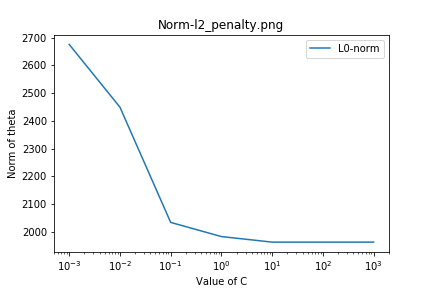
\includegraphics[width=.5\textwidth]{31e.png}\\
\indent We can see that the L0-norm of $\bar{\theta}$ decreases as $C$ increases,
but gradually converges to 2000.\\ \\
\textbf{(f)} The most positive / negative words are shown below:\\ \\
\begin{tabular}{|c|c||c|c|}
\hline
\bf Positive Coefficient & \bf Word & \bf Negative Coefficent & \bf Word\\ \hline
0.969 & thanks & -0.615 & hours \\ \hline
0.901 & thank & -0.549 & delayed \\ \hline
0.765 & great & -0.521 & due \\ \hline
0.596 & good & -0.507 & good \\ \hline
\end{tabular}\\ \\
\subsection*{3.2 Hyperparameter Selection for a Quadratic-Kernel SVM}
\textbf{(a)} The optimal parameters under different metrics are shown below:\\ Grid search: \\\\
\begin{tabular}{|c|c|c|c|}
\hline
\bf Performance Metric & \bf C & \bf r & \bf Performance \\ \hline
Accuracy & 10 & 1000 & 0.840 \\ \hline
F1-Score & 10 & 1000 & 0.839 \\ \hline
AUROC & 1000 & 0.1 & 0.918 \\ \hline
Precision & 10 & 1000 & 0.846 \\ \hline
Sensitivity & 0.001 & 0.001 & 0.948 \\ \hline
Specificity & 10 & 100 & 0.848 \\ \hline
\end{tabular}\\ \\
Random search: \\\\
\begin{tabular}{|c|c|c|c|}
\hline
\bf Performance Metric & \bf C & \bf r & \bf Performance \\ \hline
Accuracy & 136.61 & 5.077 & 0.848 \\ \hline
F1-Score & 136.61 & 5.077 & 0.846 \\ \hline
AUROC & 136.61 & 5.077 & 0.916 \\ \hline
Precision & 136.61 & 5.077 & 0.852 \\ \hline
Sensitivity & 0.0014 & 0.0033 & 0.918 \\ \hline
Specificity & 136.61 & 5.077 & 0.854 \\ \hline
\end{tabular}\\ \\
\textbf{(b)} The AUROC results are shown below:\\\\
\begin{tabular}{|c|c|c|c|}
\hline
\bf Tuning Scheme & \bf C & \bf r & \bf AUROC \\ \hline
Grid Search & 1000 & 0.1 & 0.918 \\ \hline
Random Search & 136.61 & 5.077 & 0.916\\ \hline
\end{tabular}\\\\
\indent The use of random search is generally better than grid search,
as it visits more distinct values of $C$ and $r$.
If $C$ and $r$ do not contribute equally to CV-performance
(which is usually the case), random search is more likely to get closer to
the optimal value of the predominant hyperparameter. Random search also gives more consistent results among metrics
(5 of the 6 metrics gives the same result)
\subsection*{3.3 Learning Non-linear Classifiers with a Linear-Kernel SVM}
\textbf{(a)} The quadratic kernel is $K(\bar{x},\bar{x}')=(\bar{x}\cdot \bar{x}'+r)^2$.
Suppose $\bar{x},\bar{x}'\in \mathbb{R}^d$, we can expand it as
\begin{align*}
K(\bar{x},\bar{x}')=&(\sum_{i=1}^{d}x_ix'_i+r)^2=(\sum_{i=1}^{d}x_ix'_i)^2+2(\sum_{i=1}^{d}x_ix'_i)r+r^2 \\
=& \sum_{i=1}^d (x_ix'_i)^2+2\sum_{i=1}^{d-1}\sum_{j=i+1}^d (x_ix'_i)(x_jx'_j)+2(\sum_{i=1}^{d}x_ix'_i)r+r^2 \\
=& \sum_{i=1}^d x_i^2 x'_i^2+2\sum_{i=1}^{d-1}\sum_{j=i+1}^d (x_ix_j)(x'_ix'_j)+2r(\sum_{i=1}^{d}x_ix'_i)+r^2 \\
=& \phi(\bar{x}) \phi(\bar{x}')
\end{align*}
Therefore $\phi(x)=[(x_i^2)_{i=1..d}, (\sqrt{2}x_ix_j)_{i=1..d-1, j=i+1..d}, (\sqrt{2r}x_i)_{i=1..d}, r]^T$ \\\\
\textbf{(b)} Explicit feature mappings are more flexible and always produces a valid kernel when multiplied,
while kernel functions must satisfy Mercer's Theorem.
However, explicit feature mappings can be difficult, sometimes impossible (rbf kernel) to compute,
while kernel functions can be computed much faster.

\subsection*{3.4 Linear-Kernel SVM with L1 Penalty and Squared Hinge Loss}
\textbf{(a)} The default max\_iter=1000 is not enough for convergence, and the result is undeterministic.
Among about 10 trials, AUROC varies between 0.91 and 0.92. In most cases $C=1000$ is optimal, but sometimes $C=100$.
After modifying max\_iter to 10000, the algorithm converges, but the result is still undeterministic. \\\\
\textbf{(b)} The plot is shown below:\\
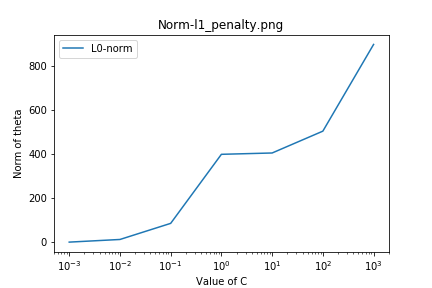
\includegraphics[width=.5\textwidth]{34b.png}\\\\
\textbf{(c)} The L1 penalty significantly decreases the L0-norm of the learned parameter.
Also, under L1 norm, the L0-norm of the learned parameter increases as $C$ increases.\\\\
\textbf{(d)} If we use Hinge Loss instead of Squared Hinge Loss, the penalty on the misclassified data points will be lighter.
More data points will become support vectors and have non-zero parameter.
Therefore, the optimal solution will have a greater L0-norm under Hinge Loss.\\
\section*{4 Asymmetric Cost Functions and Class Imbalance}
\subsection*{4.1 Arbitrary class weights}
\textbf{(a)} If $W_n$ is much greater than $W_p$, misclassified negative data points will be much more severely penalized
than misclassified positive data points. Our model will be trained to emphasize more on correctly classifying negative data points.\\\\
\textbf{(b)} The performance of the modified SVM is shown below:\\\\
\begin{tabular}{|c|c|c|}
\hline
\bf Performance Metric & \bf Performance \\ \hline
Accuracy &  0.563 \\ \hline
F1-Score &  0.222 \\ \hline
AUROC &  0.905 \\ \hline
Precision &  1.0 \\ \hline
Sensitivity &  0.125 \\ \hline
Specificity &  1.0 \\ \hline
\end{tabular}\\ \\\\
\textbf{(c)} Compared to 3.1(d), F1-score and sensitivity are affected the most.
As stated in 4.1(a), the new class weights make the model emphasize more on classifying negative data points and lowers
sensitivity, which is the metric for classifying positive data points. Since F1-score is a function of sensitivity,
it gets affected as well.
\subsection*{4.2 Imbalanced data}
\textbf{(a)} The performance of the SVM with $C=0.01$, $W_n=W_p=1$ is shown below:\\\\
\begin{tabular}{|c|c|c|}
\hline
\bf Performance Metric & \bf Performance \\ \hline
Accuracy &  0.384 \\ \hline
F1-Score &  0.374 \\ \hline
AUROC &  0.911 \\ \hline
Precision &  1.0 \\ \hline
Sensitivity &  0.23 \\ \hline
Specificity &  1.0 \\ \hline
\end{tabular}\\ \\\\
\textbf{(b)} In the imbalanced data set in this question, there are more negative points than positive points.
If we train the SVM with balanced class weights, we end up penalizing more on misclassified negative points and
make the model better at classifying negative points, as indicated by specificity=1.
However, the model performed poorly at classifying positive points, as indicated by a low sensitivity.
\subsection*{4.3 Choosing appropriate class weights}
\textbf{(a)} Since there are more negative points than positive points, metrics that evaluates the classification of both classes tend to be dominated by the majority class. The F1-score is more informative in such situation since it focuses on
classifying positive points and maintains a balance between sensitivity and precision,
which helps mitigating the situation in 4.2. \\
\indent A coarse grid search is performed first to determine a reasonable, smaller range of class weights.
After finding a smaller range, another random search is performed. Considering that in the imbalanced dataset here,
the proportion between negative and positive points is about 3:1, $W_n:W_p$ is fixed inverse-proportionally to 1:3
to further reduce the effort wasted. \\
\indent This approach gives its best results as $W_n=0.212$, $W_p=0.636$ ($C=1$),
which achieves F1-Score=0.777 in cross-validation. The corresponding test performances are shown below: \\\\
\begin{tabular}{|c|c|c|}
\hline
\bf Performance Metric & \bf Performance \\ \hline
Accuracy &  0.858 \\ \hline
F1-Score &  0.905 \\ \hline
AUROC &  0.938 \\ \hline
Precision &  0.971 \\ \hline
Sensitivity &  0.848 \\ \hline
Specificity &  0.9 \\ \hline
\end{tabular}\\ \\\\
\subsection*{4.4 The ROC curve}
\textbf{(a)} The ROC curves are shown below:\\
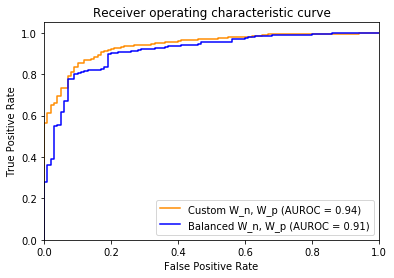
\includegraphics[width=.5\textwidth]{44.png}\\
\section*{5 Challenge}

\end{document}
